\section{Hadoop Example: wordcount}

We've prepared a dummy text file, containing \emph{lorem ipsum}, an industry standard dummy text in the printing and typesetting since 1500s. The text file contains 150 paragraphs, 13547 words, and is used to test.

The text file is transmitted to the master node via \texttt{scp} at \texttt{/root/lorem.txt}.

by running the commands below (at \texttt{/root} folder):

\begin{verbatim}
hadoop fs -mkdir /input
hadoop fs -put lorem.txt /input
hadoop jar /usr/lib/hadoop/share/hadoop/\
mapreduce/\
hadoop-mapreduce-examples-3.3.1.jar \
wordcount /input /output
hadoop fs -cat /output/part-r-00000
\end{verbatim}

The running results are shown in figure \ref{fig:word-count}. Both input file and results are put in the \texttt{WordCount} folder.

\begin{figure}[ht]
    \centering
    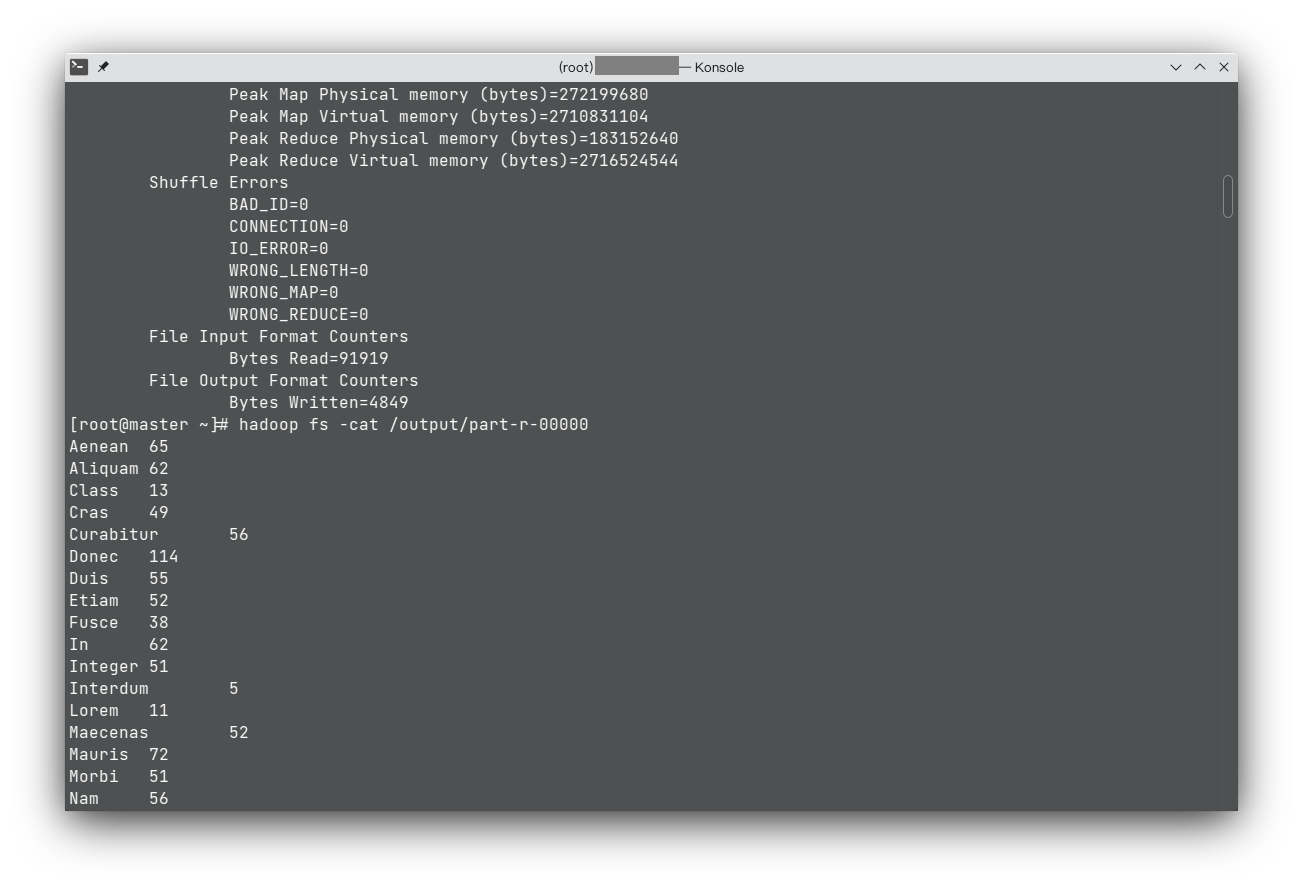
\includegraphics[width=\figurewidth]{figure/word-count.png}
    
    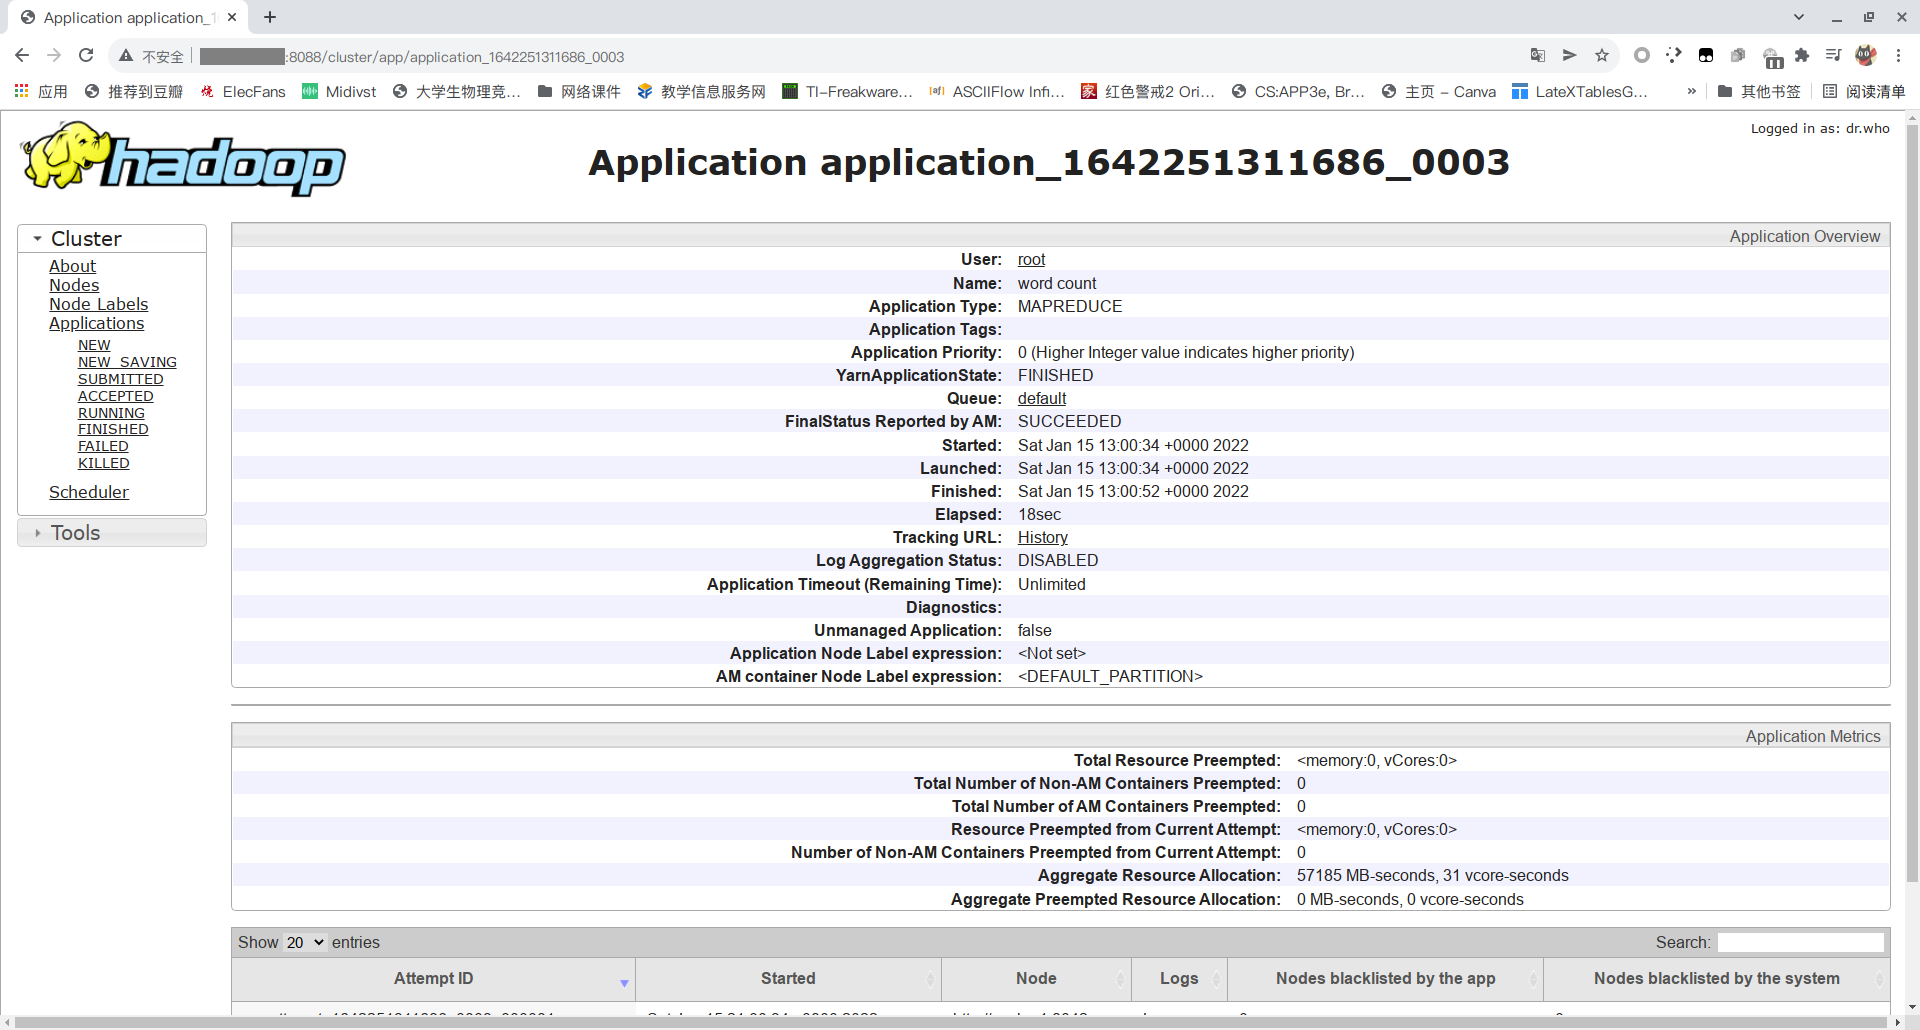
\includegraphics[width=\figurewidth]{figure/mapreduce.png}
    \caption{Word Count Results}
    \label{fig:word-count}
\end{figure}

By running the commands below, we can clear the input files and results. This will be helpful for further experiments.

\begin{verbatim}
hadoop fs -rm -f -r /output
hadoop fs -rm -f -r /input
\end{verbatim}